\documentclass{abstract_hutech}

\begin{document}
\thispagestyle{firstpage}
\twocolumn[
\begin{@twocolumnfalse}
\vspace*{20pt}
\begin{flushleft}
\fontsize{20}{0}\selectfont{\textbf{천체망원경 모터 포커서 컨트롤러 구동 시스템 개발 및 자동초점조절 알고리즘 구현}}
\vspace{32pt}\par
\fontsize{10}{12}\selectfont{\textbf{우리가 천체를 관측하기 위해서 천체망원경을 자주 사용하고는 한다. 하지만 천체망원경으로 초점을 정확하게 맞춰야지만 보다 정확한 천체관측을 진행할 수 있다. 대부분 망원경에는 이미 초점을 맞추기 위해 손으로 직접 접안렌즈의 거리를 조절하거나, 조절할 수 있는 모터를 이용해 정확하게 우리 눈으로 초점을 맞출 수 있게 만들어져 있다. 하지만, 모터를 이용하여 초점을 맞춘다고 해도 우리 눈으로 초점을 맞추는 것이기 때문에 정확하지 않을 수 있다. 본 논문에서는 아두이노를 이용하여 모터를 돌려 초점이 맞춰졌는지 관측하기 위한 구체적인 방안을 제시한다. 이뿐만이 아니라, 이를 이용하여 센서를 이용하여 자동으로 초점을 맞추는 기계를 만드는 것에 대회여 탐구하였다. 만약 이를 실현하게 한다면 천체망원경을 이용하여 여러 천체를 관측하는 데 큰 도움이 될 수 있을 것이다.
}}
\end{flushleft}
\vspace{20pt}
\end{@twocolumnfalse}
]

\section{서론}

\subsection{선정 배경}

천체를 관측할 때 초점을 맞춘다면 관측할 천체의 모습이 더 선명하게 보인다. 일반적으로 대부분의 망원경은 초점을 손으로 맞출 수 있게 설계되어있다. 하지만 모터포커서가 있다면 손으로 초점을 맞추는 것보다 정확하게 초점을 맞출 수 있게 된다. 모터 포커서와 천체 사진 분석 기술을 활용하면 사람이 손으로 초점을 맞추는 것보다 정확하게 초점을 찾을 수 있을 것이다. 그림 1, 그림 2에서 알 수 있듯이 모터포커싱을 이용하여 초점을 맞추면 아무것도 하지 않고 그냥 관측했을 때에 비해서 훨씬 정확하게 천체를 관측할 수 있게 된다. 그림 1과 그림 2를 비교하여 보면 그림 2의 표면이 훨씬 더 선명하다는 사실을 알 수 있다. 실제로 모터 포커서와 연계해 초점을 맞춰주는 오토포커싱 소프트웨어도 몇 종류가 있으나 오류가 발생하는 경우가 있다. 또한 미국 Starizona 회사에서 판매하는 오토포커싱 장치인 Micro Touch의 제품같은 경우에는 작동은 잘 하지만, 가격이 499달러로 매우 비싸다. 따라서 천체망원경의 모터 포커서의 컨트롤러 구동 시스템을 아두이노 기반으로 개발하면 여러 천체를 관측하는 데 있어서 보다 정확한 사진들을 얻을 수 있을 것이고, 가격이부담 없이 이러한 시스템을 구동할 수 있을 것이다.

\begin{figure}
\centering

\includegraphics[width=0.7\linewidth]{../../../Desktop/before}
\caption{초점을 맞추기 전의 태양 표면}
\label{fig:before}
\end{figure}

\begin{figure}
\centering
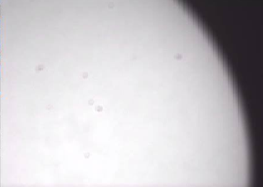
\includegraphics[width=0.7\linewidth]{../../../Desktop/after}
\caption{초점을 맞춘 후의 태양 표면}
\label{fig:after}
\end{figure}

\subsection{이론적 배경}

그림 3이 바로 Micro touch로, 시중에 나와있는 모터포커서이다. 이를 옆의 컴퓨터와 연결시킨 그림이 바로 그림4로, 이를 이용하여 컴퓨터에서도 ASCOM이라는 프로그램을 이용하여 원격으로 모터의 초점을 맞출 수 있도록 설정할 수가 있다. 그림3에서 나온 위의 두 버튼(IN, OUT)은 각각 초점을 맞추기 위해 망원경의 길이를 줄이거나 늘일 수 있는 버튼이다. Micro touch를 수동 혹은 자동으로 작동시켜 IN또는 OUT의 명령을 내렸을 경우, 그림 5에 보이는 모터포커서가 작동하게 된다. 이 모터포커서는 그림 5의 오른쪽에 보이는 모터를 움직여 천체망원경의 경통의 길이를 조절할 수 있도록 한다. 경통의 길이가 변화하면 그에 따라서 빛이 퍼지는 정도가 달라지므로 이를 잘 조정하면 망원경으로 관측하는 천체의 초점을 맞출 수 있게 된다.
\begin{figure}
\centering
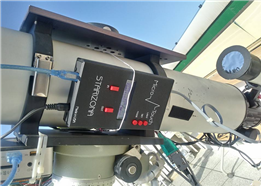
\includegraphics[width=0.7\linewidth]{../../../Desktop/telescope1}
\caption{Micro Touch를 천체망원경에 부착시킨 모습}
\label{fig:telescope1}
\end{figure}

\begin{figure}
\centering
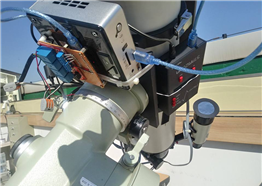
\includegraphics[width=0.7\linewidth]{../../../Desktop/telescope2}
\caption{Micro Touch와 연결된 컴퓨터}
\label{fig:telescope2}
\end{figure}

\begin{figure}
\centering
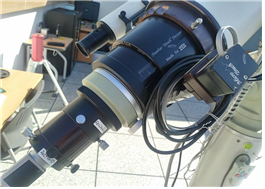
\includegraphics[width=0.7\linewidth]{../../../Desktop/telescope3}
\caption{모터포커서와 망원경의 길이}
\label{fig:telescope3}
\end{figure}

\section{연구내용 및 방법}

\subsection{아두이노를 이용한 모터 포커서 제작}

모터 포커서 컨트롤러를 만들기 위해서는 아두이노를 이용하려고 한다. 아두이노를 이용하여 모터를 제어하는 펌웨어를 짜고 프로그램을 만든다. 아두이노로 모터를 제어할 수 있는 회로를 구성한 후 모터를 연결하여 모터가 돌아갈 수 있도록 해본다.

\subsection{모터 포커서 구동 펌웨어 개발}

아두이노를 이용하여 모터 포커서에 쓰일 모터를 제어하는 코드를 만드는 데 아두이노를 이용하여 모터가 돌아가는 각도를 제어할 수 있는 프로그램을 코딩해보고 이를 모터 포커서에 연결하여 실제로 제어하는 대로 모터 포커서의 모터가 잘 작동하는지 확인한다.

\subsection{모터 포커서 ASCOM 드라이버 개발 및 컴퓨터와의 연동}

모터 포커서를 활용하기 위해서는 별의 크기를 분석해서 돌려야 하므로 컴퓨터와의 연동이 필요하다. 따라서 모터 포커서의 ASCOM 드라이버를 제작해야 한다. ASCOM 드라이버를 이용하면 카메라로부터 정보를 컴퓨터가 받아서 데이터를 분석하고, 이 분석한 데이터를 이용하여 아두이노가 어떻게 조절해야 할지 명령을 내리면 ASCOM 드라이버를 통해 정보를 전달하여 모터가 제어한 대로 조절하는 것이 가능할 것이다.

\subsection{카메라(또는 CCD) 제어 프로그램 개발}

사진 관측을 이용해서 얻은 사진을 컴퓨터로 연결하여 분석할 수 있도록 해야 한다. 그러기 위해서는 사진을 컴퓨터로 보낼 수 있어야 한다. 또한, 카메라에 나오는 화면의 변화를 보아야 하므로 연속적인 변화를 보낼 수 있는 프로그램을 만들어야 한다.

\subsection{오토 포커싱 알고리즘 개발 및 구현}

천체망원경의 초점을 맞추기 위해 사진 관측의 사진을 연속적으로 찍어서 컴퓨터로 보내주고, 컴퓨터는 이를 분석하여 모터 포커서 컨트롤러에 별의 크기가 커지고 있는지 작아지고 있는지 정보를 알고리즘에 보내준다. 그러면 프로그래밍 된 아두이노가 모터를 어느 방향으로 돌려야 하는지 판단하여 모터를 돌리고, 이 과정을 반복하여 별의 크기가 제일 작아질 때, 즉 별의 초점이 맞을 때 이 과정을 멈춘다.

\section{연구결과의 활용과 기대효과}

본 연구는 자동초점조절 알고리즘을 이용하여 모터 포커서를 구동시킴으로서 망원경으로 관측을 하는 경우나 이에 관련된 연구를 진행할 때 사람의 손으로 포커싱을 하는 것보다 정확하고 빠르게 오토모터포커싱을 할 수 있음으로서 사람들에게 편리함을 제공할 수 있고, 기존의 제품보다 더 값싸게 구현이 가능할 것이다.

Abstracts and Papers should be written according to the following order: ①Title ②Ab을stract ③Main text ④References.

\begin{thebibliography}{99}
\bibitem{한인구} 한인구, 김형국. (2009). 자동 개인 사진 분류장치. 정보 및 제어 논문집, , 105-106.
\bibitem{이덕규} 이덕규, 육영춘, 연정흠, 장수영, 이응식. (2014). 고해상도 전자광학카메라 초점조절장치 개발. 한국항공우주학회 학술발표회 초록집, , 553-555.
\bibitem{한헌수} 한헌수, 최정렬. (2004). 실시간 감시 카메라를 구현하기 위한 고속 영상확대 및 초점조절 기법. 한국정밀공학회지, 21(3), 74-82.
\end{thebibliography}

\end{document}